\documentclass[tikz]{standalone}
\usepackage{amsmath}
\definecolor{bg}{HTML}{171D2B}
\definecolor{acc}{HTML}{F7B538}
\definecolor{ln}{HTML}{8FA3BF}
\begin{document}
\pagecolor{bg}
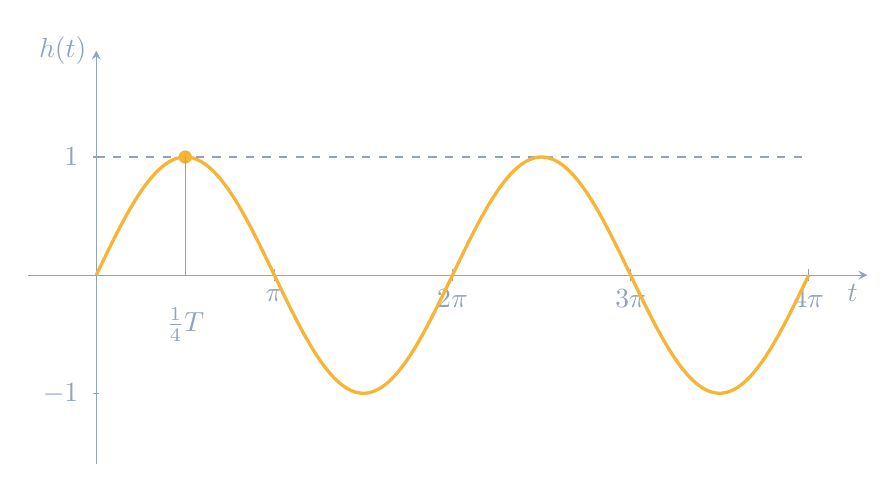
\begin{tikzpicture}[x=0.72cm,y=1.5cm,>=stealth,text=white]
  \draw[->,thin,ln] (-1.2,0) -- (13.6,0) node[below left] {$t$};
  \draw[->,thin,ln] (0,-1.6) -- (0,1.9) node[left] {$h(t)$};
  \foreach \x/\l in {3.14159/{$\pi$},6.28318/{$2\pi$},9.42478/{$3\pi$},12.56637/{$4\pi$}}
    \draw[thin,ln] (\x,-0.05) -- (\x,0.05) node[below=4pt] {\l};
  \foreach \y/\l in {-1/{$-1$},1/{$1$}}
    \draw[thin,ln] (-0.05,\y) -- (0.05,\y) node[left=4pt] {\l};
  \draw[ln,dashed,thin] (0,1) -- (12.56637,1);
  \draw[acc,very thick,domain=0:12.56637,samples=300,smooth]
    plot (\x,{sin(deg(\x))});
  \fill[acc] (1.5708,1) circle (2.4pt);
  \draw[ln,thin] (1.5708,0) -- (1.5708,1);
  \node[ln] at (1.5708,-0.42) {$\tfrac{1}{4}T$};
  \node[white] at (10.5,-1.15) {$h(t)=\sin t,\ 0\le t\le 4\pi$};
\end{tikzpicture}
\end{document}
